% TODO: Commento intervalli di confidenza
% TODO: rileggere la parte relativa ai risultati ottenuti
% TODO: rilettura
% TODO: commento sul migliore modello
% TODO: Commento sugli intervalli di confidenza in relazione agli altri modelli
% TODO: Confronto con il percettrone
\chapter{Rete neurale} \label{chp:reteNeurale}
\section{Risultati}


Fatta questa precisazione, si può procedere con la presentazione dei risultati
ottenuti. Utilizzando i dati del test set, è stato possibile valutare le
prestazioni della rete neurale addestrata. In particolare, sono state calcolate
le seguenti metriche:
\begin{itemize}
    \item Accuratezza
    \item Precisione
    \item Richiamo
    \item F1 score
\end{itemize}
Oltre al calcolo di queste metriche, si è deciso di realizzare la curva ROC per
il modello e di rappresentare la matrice di confusione. Nella tabella
\ref{tab:risultatiReteNeurale} sono presentati i risultati ottenuti dal modello
addestrato.
\begin{table}[!ht]
    \centering
    \begin{tabular}{@{}cllll@{}}
        \toprule
        \rowcolor[HTML]{EFEFEF}
        \textbf{Metrica}                        & \textbf{Accuratezza}         & \textbf{Precisione}          & \textbf{Richiamo}            & \textbf{F1 score}            \\ \midrule
        \cellcolor[HTML]{EFEFEF}\textbf{Valore} & \multicolumn{1}{c}{98.93 \%} & \multicolumn{1}{c}{98.52 \%} & \multicolumn{1}{c}{99.10 \%} & \multicolumn{1}{c}{98.81 \%} \\ \bottomrule
    \end{tabular}
    \caption{Risultati ottenuti dal modello addestrato}
    \label{tab:risultatiReteNeurale}
\end{table}

Dai valori riportati nella tabella \ref{tab:risultatiReteNeurale} si può notare
che la rete neurale ha ottenuto dei valori delle metriche molto alti. Questo
comportamento è giustificato dal fatto che in fase di analisi è stato possibile
notare che le feature selezionate sono in grado di discriminare in modo efficace
le due classi.

In aggiunta al calcolo di queste metriche, è stata calcolata la matrice di confusione
per il modello addestrato. La matrice di confusione ottenuta è riportata in figura
\ref{fig:matriceConfusioneReteNeurale}.

\begin{figure}[!ht]
    \centering
    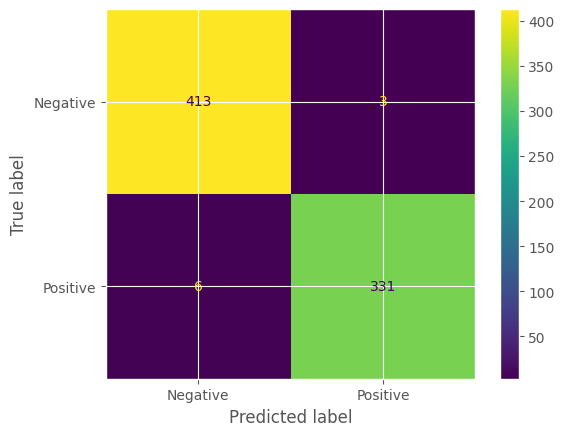
\includegraphics[width=0.5\textwidth]{img/rete/matrice_confusione.png}
    \caption{Matrice di confusione ottenuta dal modello addestrato}
    \label{fig:matriceConfusioneReteNeurale}
\end{figure}

Dalla matrice di confusione è possibile confermare i risultati ottenuti dalle
metriche calcolate in precedenza. Inoltre, avendo corretto manualmente il valore
della soglia, si è riusciti a ridurre il numero di falsi negativi, il che ha
permesso di aumentare il valore del richiamo.

Per concludere questa prima parte di analisi dei risultati, è stata realizzata
la curva ROC per il modello addestrato. La curva ROC ottenuta è riportata in
figura \ref{fig:curvaRocReteNeurale}. Oltre alla curva ROC è stata calcolata
l'area sotto la curva, la quale ha ottenuto un valore di $1.00$. Questo valore
ci permette di affermare che il modello addestrato si avvicina molto alla
perfetta classificazione.

\begin{figure}[!ht]
    \centering
    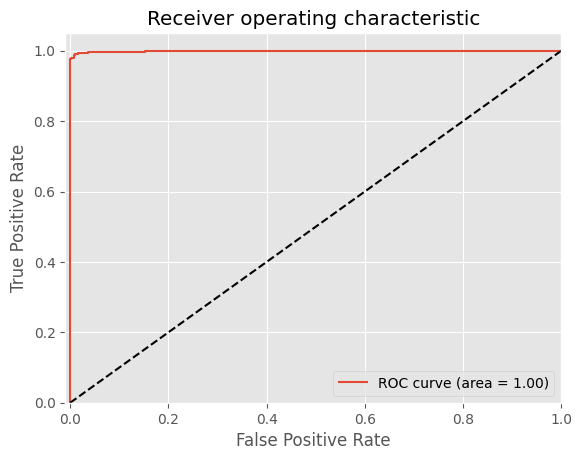
\includegraphics[width=0.8\textwidth]{img/rete/curva_roc.png}
    \caption{Curva ROC ottenuta dal modello addestrato}
    \label{fig:curvaRocReteNeurale}
\end{figure}
\subsection*{K-fold validation}
Per avere una visione più chiara dei risultati ottenuti, si è deciso di effettuare
una valutazione del modello attraverso 10 fold di cross validation. In questo
processo ogni modello che è stato addestrato è stato valutato attraverso le
metriche di accuratezza, precisione, richiamo e F1 score.

Per svolgere questa operazione è stato utilizzato il dataset completo, ovvero
senza alcuna suddivisione in training set e test set.

Anche per questa operazione è stato utilizzato il valore di threshold precedentemente
definito, ovvero $0.3$.

Sui risultati ottenuti da questo processo sono stati calcolati gli intervalli
di confidenza al $90\%$. I risultati ottenuti sono riportati in tabella
\ref{tab:risultatiCrossValidation}.

\begin{table}[ht]
    \centering
    \begin{tabular}{@{}lcc@{}}
        \toprule
        \rowcolor[HTML]{EFEFEF}
        \multicolumn{1}{c}{\cellcolor[HTML]{EFEFEF}\textbf{Metrica}} & \textbf{Valore Medio} & \textbf{Intervallo di confidenza} \\ \midrule
        Accuratezza                                                  & 98.27 \%              & [97.98\%, 98.55\%]                \\
        Precisione                                                   & 97.99 \%              & [97.47\%, 98.52\%]                \\
        Richiamo                                                     & 98.15 \%              & [97.49\%, 98.81\%]                \\
        F1 score                                                     & 98.06 \%              & [97.75\%, 98.38\%]                \\ \bottomrule
    \end{tabular}
    \caption{Risultati ottenuti dalla cross validation}
    \label{tab:risultatiCrossValidation}
\end{table}

Gli intervalli ottenuti sono stati successivamente rappresentati in un grafico
riportato in figura \ref{fig:risultatiCrossValidation}. Questo grafico permette
di avere una visione più chiara dei risultati ottenuti dalla cross validation.

\begin{figure}[!ht]
    \centering
    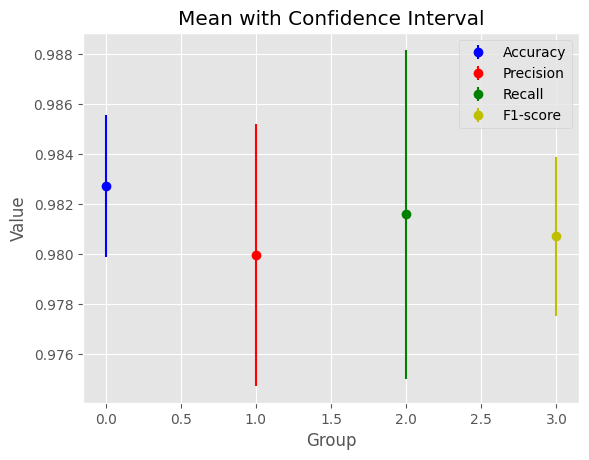
\includegraphics[width=0.5\textwidth]{img/rete/intervalli_confidenza.png}
    \caption{Risultati ottenuti dalla cross validation}
    \label{fig:risultatiCrossValidation}
\end{figure}
\section{Modello addestrato con PCA}
\subsection{Risultati}
Addestrato il modello con i dati ottenuti attraverso la PCA, si è proceduto con
la valutazione delle prestazioni del modello utilizzando le stesse metriche
utilizzate in precedenza e il test set.

I risultati ottenuti dal modello addestrato con la PCA sono riportati in tabella
\ref{tab:risultatiReteNeuralePCA} e sono confrontati con quelli ottenuti dal
modello addestrato con le feature selezionate manualmente.

\begin{table}[ht]
    \centering
    \begin{tabular}{@{}lccccc@{}}
        \toprule
        \rowcolor[HTML]{EFEFEF}
        \multicolumn{1}{c}{\cellcolor[HTML]{EFEFEF}\textbf{Modello}} & \textbf{Accuratezza} & \textbf{F1} & \textbf{Precision} & \textbf{Recall} \\ \midrule
        Rete senza PCA                                               & 98.80\%              & 98.65\%     & 99.10\%            & 98.65\%         \\
        Rete con PCA                                                 & 98.27\%              & 98.07\%     & 97.92\%            & 98.21\%         \\ \bottomrule
    \end{tabular}
    \caption{Risultati ottenuti dai modelli addestrati con PCA}
    \label{tab:risultatiReteNeuralePCA}
\end{table}

Dai valori riportati nella tabella \ref{tab:risultatiReteNeuralePCA} si può notare
che il modello addestrato con le feature selezionate manualmente ha ottenuto
dei risultati migliori rispetto a quello addestrato con la PCA.

È stata anche calcolata la matrice di confusione per il modello addestrato con
la PCA. La matrice di confusione ottenuta è riportata in figura \ref{fig:matriceConfusioneReteNeuralePCA}.

\begin{figure}[!ht]
    \centering
    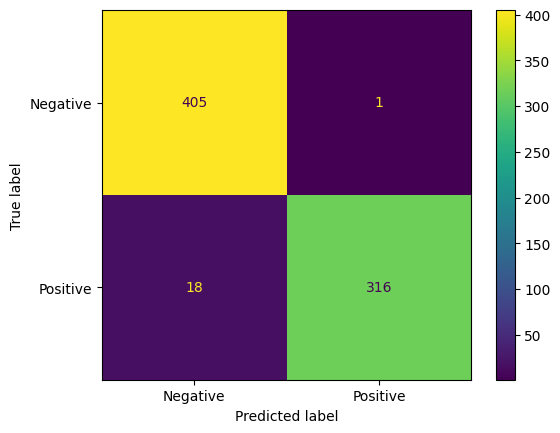
\includegraphics[width=0.5\textwidth]{img/rete/matrice_confusione_pca.png}
    \caption{Matrice di confusione ottenuta dal modello addestrato con PCA}
    \label{fig:matriceConfusioneReteNeuralePCA}
\end{figure}

In aggiunta a queste metriche, i modelli sono stati confrontati attraverso la
10-fold cross validation. I risultati ottenuti sono riportati in tabella
\ref{tab:risultatiCrossValidationPCA}.

\begin{table}[ht]
    \centering
    \resizebox{\textwidth}{!}{\begin{tabular}{@{}lccc@{}}
        \toprule
        \rowcolor[HTML]{EFEFEF}
        \multicolumn{1}{c}{\cellcolor[HTML]{EFEFEF}\textbf{Metrica}} & \textbf{Valore Medio} & \textbf{Intervallo di confidenza con PCA} & \textbf{Intervallo di confidenza senza PCA} \\ \midrule
        Accuratezza                                                  & 98.35 \%              & [97.97\%, 98.72\%]                        & [97.98\%, 98.55\%]                          \\
        Precisione                                                   & 98.05 \%              & [97.51\%, 98.58\%]                        & [97.47\%, 98.52\%]                          \\
        Richiamo                                                     & 98.27 \%              & [97.62\%, 98.93\%]                        & [97.49\%, 98.81\%]                          \\
        F1 score                                                     & 98.15 \%              & [97.73\%, 98.58\%]                        & [97.75\%, 98.38\%]                          \\ \bottomrule
    \end{tabular}}
    \caption{Risultati ottenuti dalla cross validation}
    \label{tab:risultatiCrossValidationPCA}
\end{table}

Oltre a confrontare le performance dei modelli utilizzando le metriche, si
è deciso di confrontare le curve ROC dei due modelli. I risultati ottenuti sono
riportati in figura \ref{fig:confrontoRisultatiPCA}.

\begin{figure}[!ht]
    \centering
    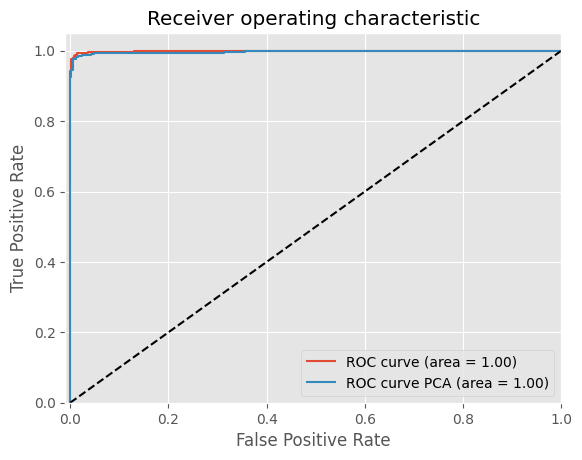
\includegraphics[width=0.8\textwidth]{img/rete/confrontoRoc.png}
    \caption{Confronto curve ROC tra il modello addestrato con e senza PCA}
    \label{fig:confrontoRisultatiPCA}
\end{figure}

Da questa figura si può notare che la differenza tra i due modelli è minima.
Entrambi i modelli si avvicinano molto alla perfetta classificazione. Si può
notare una differenza maggiore tra i due modelli osservando gli intervalli di
confidenza. In particolare, si riesce a osservare una differenza di ampiezza
degli intervalli di confidenza tra i due modelli.

Il modello ottenuto attraverso la PCA ha un intervallo di confidenza più ampio
rispetto a quello ottenuto senza PCA, anche se il valore medio delle metriche
è leggermente superiore nel caso di PCA.

Nella figura \ref{fig:intervalliConfidenzaPCA} sono riportati gli intervalli di
confidenza ottenuti dai modelli addestrati con e senza PCA. Da questa figura si
può notare che l'intervallo di confidenza ottenuto dal modello addestrato con
PCA, rappresentato dalla linea di colore rosso, è più ampio rispetto a quello
ottenuto dal modello addestrato senza PCA, rappresentato dalla linea di colore blu.
\begin{figure}[!ht]
    \centering
    \begin{subfigure}[b]{0.4\textwidth}
        \centering
        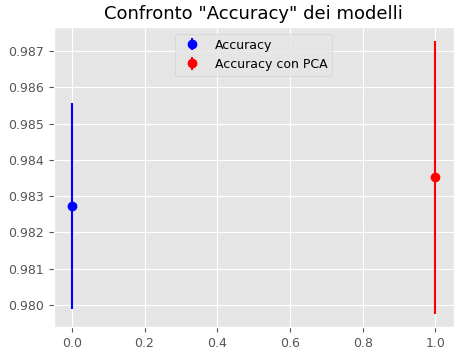
\includegraphics[width=\textwidth]{img/rete/intervalliAcc.png}
        \caption{Accuracy}
        \label{fig:acc}
    \end{subfigure}
    \hfill
    \begin{subfigure}[b]{0.4\textwidth}
        \centering
        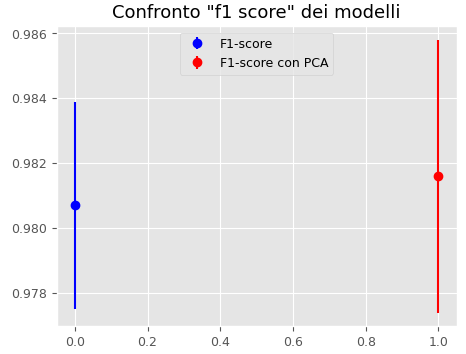
\includegraphics[width=\textwidth]{img/rete/intervalliF1.png}
        \caption{F1 score}
        \label{fig:f1}
    \end{subfigure}
    \hfill
    \begin{subfigure}[b]{0.4\textwidth}
        \centering
        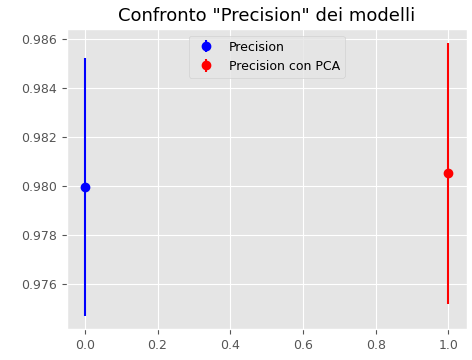
\includegraphics[width=\textwidth]{img/rete/intervalliPrecision.png}
        \caption{Precision}
        \label{fig:precision}
    \end{subfigure}
    \hfill
    \begin{subfigure}[b]{0.4\textwidth}
        \centering
        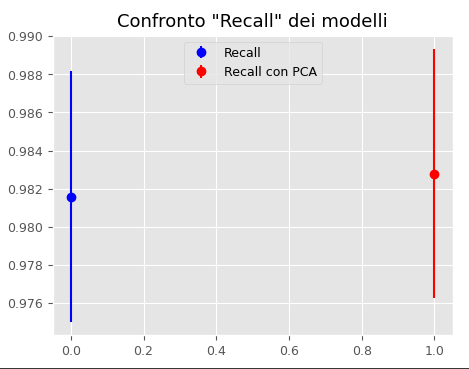
\includegraphics[width=\textwidth]{img/rete/intervalliRecall.png}
        \caption{Recall}
        \label{fig:recall}
    \end{subfigure}
    \caption{Intervalli di confidenza ottenuti dai modelli addestrati con e senza PCA}
    \label{fig:intervalliConfidenzaPCA}
\end{figure}
